\documentclass{cmspaper}
\usepackage{lineno}
\usepackage{amsfonts,amsmath,amssymb}
\usepackage[dvips]{graphicx}
\usepackage{bm}
\usepackage{multirow}
\usepackage{subfigure}  % use for side-by-side figures
%\usepackage[a4paper]{hyperref}

\def\etmiss{\big\slash\hspace{-1.6ex}{E_\text{T}}}
\def\etmissB{\big\slash\hspace{-1.6ex}{\boldsymbol{E}_\text{T}}}
\def\exmiss{\big\slash\hspace{-1.6ex}{E_{x}}}
\def\eymiss{\big\slash\hspace{-1.6ex}{E_{y}}}
\def\sumet{\sum{E_\text{T}}}
\def\sumetB{\sum{\boldsymbol{E}_\text{T}}}

\begin{document}
\begin{linenumbers}


\begin{titlepage}

  % select one of the following and type in the proper number:

%  \cmsnote{2010/001}
  \internalnote{2005/000}
%  \conferencereport{2005/000}
%  \cmsan{2010/029}
%  \cmsdtnote{2005/000}
%  \cmspas{2005/000}
   \date{\today}

  \title{Results of visual scan of high $\etmiss$ events in 7 TeV pp collision data}

  \begin{Authlist}
    A.~Apresyan
    \Instfoot{caltech}{California Institute of Technology, Pasadena, CA, USA}
    D.~Ferencek, F.~Santanastasio %\Aref{a}
   \Instfoot{umd}{University of Maryland, College Park, MD, USA}   
  \end{Authlist}

% if needed, use the following:
%\collaboration{CMS collaboration}

%\Anotfoot{a}{Also at \textit{California Institute of Technology, Pasadena, CA, USA}}

  \begin{abstract}    
   We present the results of a visual scan of high $\etmiss$ events 
   (Calo$\etmiss>45$~GeV OR tc$\etmiss>45$~GeV OR pf$\etmiss>45$~GeV)
   in a sample of 12~nb$^{-1}$ of 7 TeV pp collision data, 
   after applying the official noise clean-up. 
   The CMS software {\it Fireworks} has been used to produce the event displays. 
   The high $\etmiss$ events have been visually inspected and classified in different 
   cathegories. The resuls of this scan can be used to further improve the noise 
   cleaning algorithms and identify possible problems in the three algorithms employed 
   in CMS for the $\etmiss$ reconstruction.
  \end{abstract} 

% if needed, use the following:
%\conference{Presented at {\it Physics Rumours}, Coconut Island, April 1, 2005}
%\submitted{Submitted to {\it Physics Rumours}}
%\note{Preliminary version}
  
\end{titlepage}

\setcounter{page}{2}%JPP

\tableofcontents

\clearpage

\section{Introduction}

Commissioning studies performed with test beams, cosmic runs and 
early 0.9~TeV, 2.36~TeV and 7~TeV pp 
collision data have identified several sources of anomalous noise 
(i.e. noise not produce solely from expected fluctuations in the electronics)
in the calorimeters of the CMS experiment:
\begin{itemize}
\item {\it ECAL barrel spikes} - More details are available at XXX.
%Energy deposits in individual channels 
%affected by the noise are cleaned using both topological and 
%timing information of the reconstructed hits. This type of noise is correlated with collisions. 

\item {\it HF PMT hits} - More details are available at~\cite{Chatrchyan:1225105},XXX.
%Energy deposits in individual channels 
%affected by the noise are cleaned using both topological and 
%timing information of the reconstructed hits. PMT hit noise is correlated with collisions. 

\item {\it IonFeedback/HPD/RBX noise in HCAL barrel and endcaps} - More details are available at XXX.
%Events with identified 
%HPD/RBX noise are removed from the analysis using a filter based on both topological 
%and timing information of the reconstructed energy deposits. IonFeedback noise has also been observed 
%but typically affect a few channels and produces low energy signals. A cleaning for IonFeedback noise 
%is not yet available. HPD/RBX noise is not correlated with collisions. 
\end{itemize}
In addition, machine-induced background, in the form of 
beam halo [XXX] and beam scraping events [XXX], have been observed. 

The overlap of either anomalous noise or machine-induced background 
with a pp collision event produces an unbalance in 
the reconstructed missing transverse energy in the event, which can produce 
large tails in the $\etmiss$ distribution. 

We present the results of a visual scan of high $\etmiss$ events 
(tc$\etmiss>60$~GeV OR pf$\etmiss>60$~GeV)
in an inclusive sample of XX~nb$^{-1}$ of 7 TeV pp collision data, 
after applying the official noise clean-up available in CMSSW\_3\_7\_0\_patch2.
The full selection criteria are described in Section~\ref{sec:EventSelection}). 
The scan is performed separately for events with tc$\etmiss>60$~GeV and pf$\etmiss>60$~GeV
since the noise clean-up is implemented differently in the two $\etmiss$ algorithms.
The CMS software {\it Fireworks} [XXX] has been used to produce the event displays. 
The high $\etmiss$ events have been visually inspected and classified in different 
categories. The results of this scan can provide hints to further improve the noise 
cleaning and to identify possible problems and inconsistencies in the algorithms employed 
in CMS for the $\etmiss$ reconstruction.


\section{Datasample, Event Selection, and Noise Cleaning} \label{sec:EventSelection}

{\bf Dataset and CMSSW release:}
\begin{itemize}
\item dataset: /MinimumBias/Commissioning10-GOODCOLL-Jun9thSkim\_v1/RECO
\item CMSSW release: CMSSW\_3\_7\_0\_patch2
\end{itemize}

{\bf Event selection:}
\begin{itemize}
\item Physics declared bit
\item BPTX bit 0
\item Removal of events with large pixel cluster multiplicity
\item Good primary vertex
\item Good Run/LS selection. JSON file: Cert\_132440-136119\_7TeV\_May27thReReco\_Collisions10\_JSON.txt  
\end{itemize}
%More details at [XXX].

{\bf Noise cleaning}

Noise cleaning/event filter for calotower-based $\etmiss$ algorithms (Calo$\etmiss$ and tc$\etmiss$):
\begin{itemize}
\item ECAL barrel spikes (reject RecHits): topology (kWeird flag = swiss cross variable) + timing (kOutOfTime flag)~\cite{ECALAt7TeV};
\item HF PMT hits (reject Rechits): topology (HFLongShort flag = PET+S9/S1) + pulse shape (HFDigiTime flag)~\cite{HFDN};
\item HPD/RBX noise in HBHE (reject events): combination of pulse shape and topological variables~\cite{HCALWGNOTE}.
\end{itemize}

Noise cleaning (reject RecHits) for pf$\etmiss$ is described at~\cite{PFPAS2010}. Timing and topology are used to reject RecHits 
affected by ECAL and HF noise. Topology only is used to reject rechits affected by HBHE noise. No events are rejected.

NOTE: The HPD/RBX noise filter is applied for the scan of both tc$\etmiss$ and pf$\etmiss$ tails presented in this note, 
in order to have the same number of events passing the selection.

Figure~\ref{fig:calomet} shows the cleaned tc$\etmiss$ and pf$\etmiss$ distributions for $\approx 60$~M events 
(precisely 58821832 events) passing the event selection described above.
\begin{figure}[h]
 \centering
 \begin{tabular}{ll}
   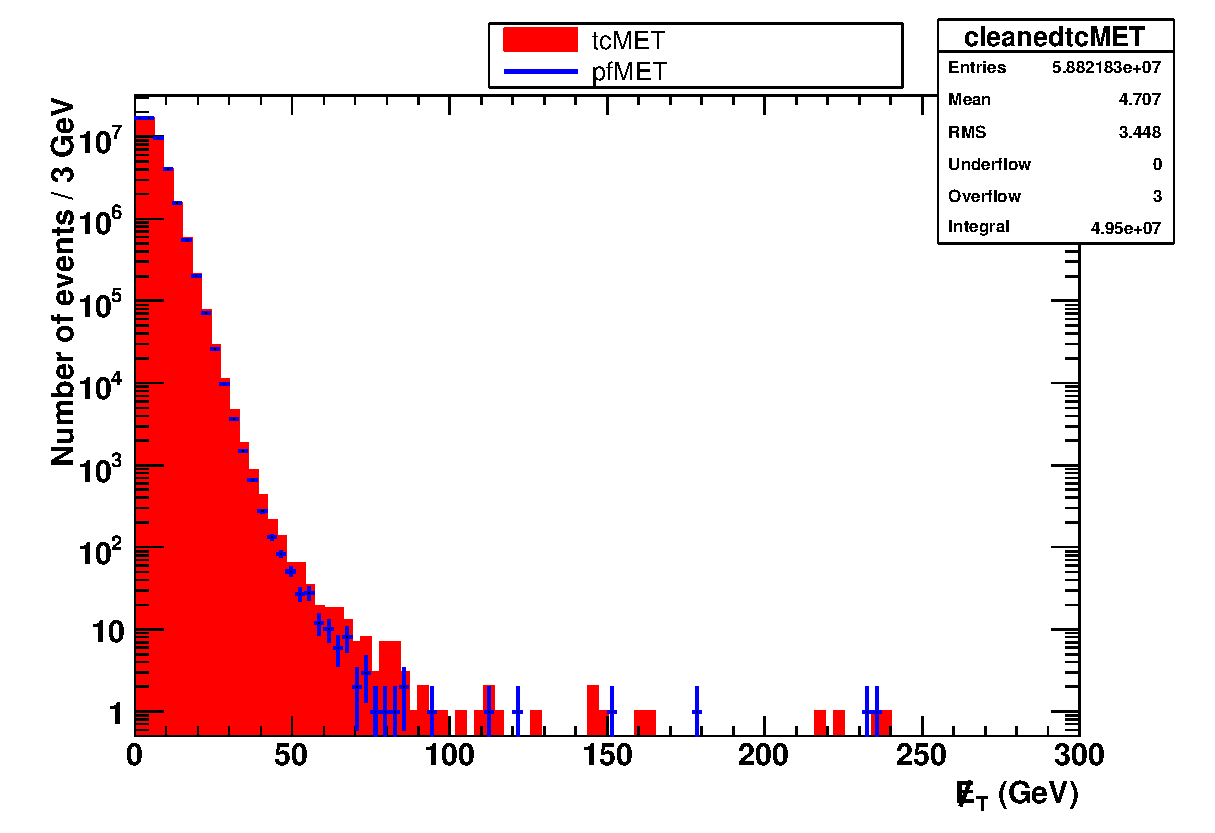
\includegraphics[width=0.7\textwidth]{fig/met.eps} 
 \end{tabular}
\caption{tc$\etmiss$ and pf$\etmiss$ distributions of 7 TeV collision data after applying the full event selection and noise cleaning.}
\label{fig:calomet}
\end{figure}

\section{Scan of high $\etmiss$ events}

The high $\etmiss$ events have been divided in three mutually exclusive categories and stored in the directory \\ 
SKIMDIR = /castor/cern.ch/user/s/santanas/MET/Skims/METtails\_45GeVcut\_May27\_2010/ :
\begin{itemize}
\item Category 1 \quad - \quad Calo$\etmiss>45$~GeV \quad AND \quad tc$\etmiss>45$~GeV\\ 
Root file in RECO format at: \\ SKIMDIR/picked\_events\_CaloMET\_and\_tcMET\_gt\_45GeV\_Artur.root
\item Category 2 \quad - \quad Calo$\etmiss>45$~GeV \quad AND \quad tc$\etmiss<45$~GeV \\
Root file in RECO format at: \\ SKIMDIR/picked\_events\_CaloMET\_gt\_45GeV\_Artur.root
\item Category 3 \quad - \quad Calo$\etmiss<45$~GeV \quad AND \quad tc$\etmiss>45$~GeV \\
Root file in RECO format at: \\ SKIMDIR/picked\_events\_tcMET\_gt\_45GeV\_Artur.root
\end{itemize}

A visual scan of these events have been performed using the CMS event display
software ``Fireworks''. It should pointed out that the results of a visual scan 
are subject to personal judgment. Nevertheless, they should provide
with good approximation a realistic picture of which are the events that populates the tails
of the $\etmiss$ after applying the current noise clean-up.

The result of the scan are summarized in the following sub-sections.

\subsection{Category 1: Calo$\etmiss>45$~GeV AND tc$\etmiss>45$~GeV}

\subsection{Category 2: Calo$\etmiss>45$~GeV AND tc$\etmiss<45$~GeV}

\subsection{Category 3: Calo$\etmiss<45$~GeV AND tc$\etmiss>45$~GeV}
%\input{Conclusion}


\end{linenumbers}
\end{document}

